\documentclass{article}
\usepackage{tikz}
\usepackage{tikz-qtree}
\newcommand{\lens}{\leftrightarrow}
\begin{document}
{\noindent\large Daniel Wagner}\\[3ex]

The problem of synchronization is ubiquitous in computing applications. In
the database community, the so-called view-update problem involves keeping a
database and the result of a query to that database in sync as updates occur
to the database and to the query's result. In large software systems, two
applications often want to share data, but have disparate preferences for
file format; or, various applications, all attempting to solve the same
problem, may want to share user data. (For example, browsers like Internet
Explorer, Firefox, and Chrome often have facilities for importing bookmarks
from their competitors.) Users with multiple computers may wish to
synchronize directory hierarchies among their computers. Large websites
often offer programming interfaces that can be modeled as presenting a
small, modifiable view of their large set of data. Even a single program
running on a single computer often keep various in-memory data structures
storing related data, and maintain synchronization invariants between the
structures. I work towards the goal of making the maintenance of
synchronized data as painless as possible, so that ephemeral data structures
and persistent data alike can benefit from formal correspondence guarantees.

There is a fair amount of preexisting work on this problem. The database
community in particular has a significant body of work on the problem of
synchronizing relational data. The framework of asymmetric lenses aims to
extend these ideas to other familiar data structures often available in
programming languages (with varying but often fairly extensive language
integration), such as strings and algebraic data types.
% TODO: citations, more expansive related work

One key property of lenses is that they are compositional: while creating a
lens for a large and complicated transformation, one can create smaller
lenses doing easy-to-understand portions of the transformation and combine
them together to perform the entire transformation. For example, consider
the problem of turning a directory tree with file name, metadata, and file
content information into a flat listing of only the text files, that is,
turning something like

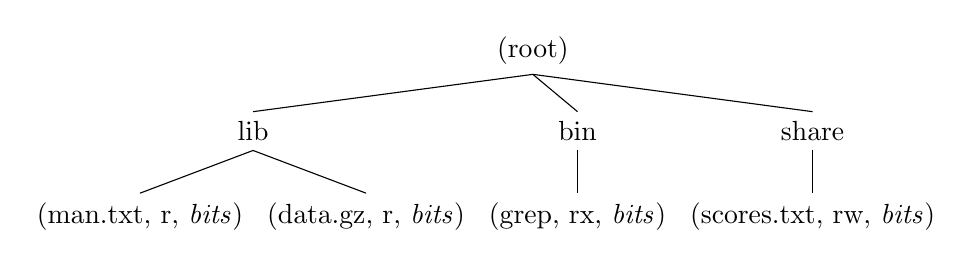
\begin{tikzpicture}
    \Tree [.(root)
        [.lib (man.txt,\ r,\ \emph{bits}) (data.gz,\ r,\ \emph{bits}) ]
        [.bin (grep,\ rx,\ \emph{bits}) ]
        [.share (scores.txt,\ rw,\ \emph{bits}) ]
    ]
\end{tikzpicture}

\noindent into a flat list like [man.txt, scores.txt]. This can be broken
into several phases: first, write a lens that synchronizes triples with a
single one of their fields $(a,b,c) \lens a$; then use vertical composition
to turn this into a lens that runs on each element of a list $[(a,b,c)]
\lens [a]$; then use horizontal composition with a lens that partitions
lists $[a+b] \lens ([a],[b])$ to turn it into a lens that filters out
directories $[(a,b,c)+d] \lens [a]$; then use horizontal composition again
with a lens that flattens trees $\mathit{Tree}\ a \lens [a]$ to turn it into
a lens that does the entire transformation $\mathit{Tree}\ ((a,b,c)+d) \lens
[a]$.
% TODO: this explanation needs a lot of work

Another key property is that the data structures being synchronized need not
store exactly the same data: some data may be available in only one of the
structures. Returning to the example above, the directory structure, file
metadata, and file contents are all missing from the list of file names.
There are various techniques for restoring this information during
synchronization, but the ability to do so is common to all frameworks.
However, there is an asymmetry in the example: only one of the two
structures has ``extra'' information. The flattened list can always be
exactly reproduced, given the directory hierarchy.

Until recently, it was believed that being symmetric -- allowing data to be
missing from both structures -- was incompatible with allowing horizontal
composition. Many frameworks with one or the other exist; however, only
recently we have shown that it is possible to marry both desirable traits in
one formalism.

I am interested in pushing this formalism forward in a variety of
directions. Most recently, we have been considering how to extend the
framework to consider not only the process of transforming one data
structure into another, but also to carefully consider what it means to edit
a data structure in a single format. A well-designed collection of edits
should allow a lens to be more efficient (by consisting of edit descriptions
which are significantly smaller than the data structure they are acting on)
and more precise (by containing more precise information about how one
version of a structure arises from another than is available by simply
presenting the two versions at once).

We have the beginnings of a formalism for lenses which act on edits, and
there are a wide variety of open problems in that area -- see my one-year
plan for an outline of the most exciting directions to push on.
\end{document}
